\documentclass[sn-mathphys,Numbered]{sn-jnl}% Math and Physical Sciences Reference Style

\usepackage{graphicx}%
\usepackage{multirow}%
\usepackage{amsmath,amssymb,amsfonts}%
\usepackage{amsthm}%
\usepackage{mathrsfs}%
\usepackage[title]{appendix}%
\usepackage{xcolor}%
\usepackage{textcomp}%
\usepackage{manyfoot}%
\usepackage{booktabs}%
\usepackage{algorithm}%
\usepackage{algorithmicx}%
\usepackage{algpseudocode}%
\usepackage{listings}%
\usepackage{tikz}%
\usetikzlibrary{shapes.geometric, arrows, positioning}

\tikzset{
    block/.style={rectangle, draw, fill=blue!10, text width=12em, text centered, rounded corners, minimum height=2.5em},
    decision/.style={diamond, draw, fill=green!10, text width=8em, text centered, minimum height=2.5em, inner sep=0pt},
    arrow/.style={thick,->,>=stealth}
}

\begin{document}

\title[Explainable Clinical Decision Support (X-CDS)]{Explainable Clinical Decision Support (X-CDS): Mitigating LLM Hallucinations in High-Stakes Medicine via Hybrid Retrieval and Deterministic Citation Verification Frameworks}

\author*[1]{\fnm{Sahil} \sur{Kumar}}\email{sahil.kumar2023@vitbhopal.ac.in}
\author[1]{\fnm{Abdul} \sur{Rahman}}\email{abdul.rahman@vitbhopal.ac.in}

\affil*[1]{\orgdiv{School of Computer Science and Engineering (SCSE)}, \orgname{VIT Bhopal University}, \orgaddress{\city{Bhopal}, \state{Madhya Pradesh}, \country{India}}}

\abstract{Large Language Models (LLMs) show significant promise in clinical decision support systems (CDSS). However, the propensity of generative models to ``hallucinate''---generate medically incorrect or unsubstantiated claims---remains a critical barrier to clinical deployment. This paper introduces \textbf{Explainable Clinical Decision Support (X-CDS)}, an architecture designed to improve the automated faithfulness of clinical recommendations via deterministic citation verification. X-CDS integrates a \textbf{Hybrid Retrieval} pipeline (ChromaDB Vector Search and BM25 Keyword Search) merged via \textbf{Reciprocal Rank Fusion (RRF)} and filtered through a \textbf{Cross-Encoder Re-ranker}. To mitigate hallucinations, we implement a stateful \textbf{LangGraph} orchestration loop that programmatically validates generative assertions against retrieved source passages using a token-overlap alignment threshold. If the generator fails validation, the state machine routes the failure back for iterative self-correction. We evaluate the system using the \textbf{Ragas} benchmarking framework against a clinical dataset, measuring Faithfulness, Answer Relevancy, Context Precision, and Context Recall. Our results demonstrate that deterministic citation guardrails significantly improve model faithfulness compared to standard RAG baselines, demonstrating the value of structured self-correction loops for safety-critical clinical applications.}

\keywords{Clinical Decision Support, Large Language Models, Hallucination Mitigation, LangGraph, Ragas Benchmarking, Hybrid Retrieval}

\maketitle

\section{Introduction}\label{sec1}
The deployment of Large Language Models (LLMs) such as GPT-4 and Gemini in clinical settings has demonstrated their potential to assist clinicians with diagnostic suggestions, literature summaries, and treatment plan generation. Despite these capabilities, generative models are fundamentally statistical next-token predictors. Consequently, they suffer from the ``hallucination'' phenomenon---generating logical-sounding but factual fabrications. In high-stakes clinical settings, an unsubstantiated treatment or diagnostic suggestion can lead to severe adverse patient outcomes.

\subsection{The Arbovirus Differential Diagnosis Dilemma}
To evaluate X-CDS in a highly challenging and clinically realistic scenario, we focus on emerging arboviruses: \textbf{Zika, Dengue, Chikungunya, and West Nile Virus}. Differentiating these pathogens represents a classic diagnostic challenge in tropical medicine due to their overlapping acute presentations (fever, rash, and joint pain). 

However, misdiagnosis carries extreme clinical risk:
\begin{itemize}
    \item A patient presenting with severe joint pain may be diagnosed with Chikungunya and prescribed non-steroidal anti-inflammatory drugs (NSAIDs) like Aspirin or Ibuprofen for pain relief.
    \item If the patient actually has Dengue, administering NSAIDs can impair platelet function and trigger severe, potentially fatal internal hemorrhages (Dengue Hemorrhagic Fever).
    \item Similarly, misdiagnosing Zika in pregnant patients can lead to missed screening opportunities for microcephaly and Congenital Zika Syndrome (CZS).
\end{itemize}

This environment perfectly simulates the high-stakes clinical scenarios where LLM hallucinations or slight inaccuracies are unacceptable. Traditional Retrieval-Augmented Generation (RAG) mitigates this by injecting relevant medical literature into the model's prompt context. However, standard RAG still fails if:
\begin{enumerate}
    \item The retrieval pipeline fails to capture critical clinical facts (poor recall).
    \item The generator ignores the injected context or synthesizes claims that lack an explicit source citation (hallucination).
\end{enumerate}

To address these vulnerabilities, we present the \textbf{X-CDS} framework. The primary contributions of this paper are:
\begin{enumerate}
    \item A dual-channel \textbf{Hybrid Retrieval} pipeline combining dense vector embeddings and sparse keyword indices merged via Reciprocal Rank Fusion (RRF) and optimized using a transformer-based Cross-Encoder re-ranker.
    \item A stateful \textbf{LangGraph Self-Correction} workflow that programmatically checks citation alignment using character-level token-overlap algorithms.
    \item An empirical evaluation of the pipeline's effectiveness using the Ragas metric framework, proving that programmatic self-correction loops maximize factual safety.
\end{enumerate}

\section{System Architecture and Methodology}\label{sec2}

\begin{figure}[htbp]
\centering
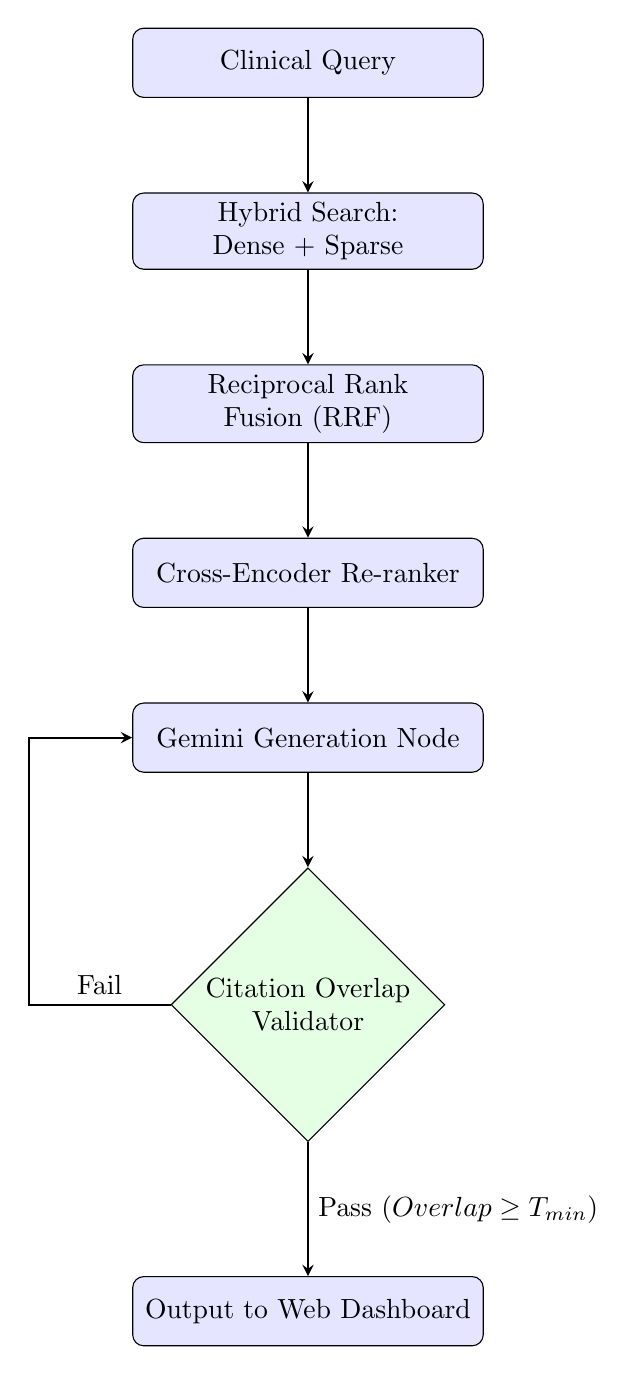
\begin{tikzpicture}[node distance = 1.2cm, auto, >=stealth]
    % Place nodes
    \node [block] (query) {Clinical Query};
    \node [block, below=of query] (hybrid) {Hybrid Search: Dense + Sparse};
    \node [block, below=of hybrid] (rrf) {Reciprocal Rank Fusion (RRF)};
    \node [block, below=of rrf] (rerank) {Cross-Encoder Re-ranker};
    \node [block, below=of rerank] (generator) {Gemini Generation Node};
    \node [decision, below=of generator] (guard) {Citation Overlap Validator};
    \node [block, below=of guard, yshift=-0.5cm] (output) {Output to Web Dashboard};
    
    % Draw edges
    \draw [arrow] (query) -- (hybrid);
    \draw [arrow] (hybrid) -- (rrf);
    \draw [arrow] (rrf) -- (rerank);
    \draw [arrow] (rerank) -- (generator);
    \draw [arrow] (generator) -- (guard);
    \draw [arrow] (guard) -- node [right] {Pass ($Overlap \ge T_{min}$)} (output);
    \draw [arrow] (guard.west) -- ++(-1.8cm,0) node [above, pos=0.5] {Fail} |- (generator.west);
\end{tikzpicture}
\caption{Stateful self-correcting clinical diagnostic pipeline architecture.}
\label{fig1}
\end{figure}

\subsection{Data Ingestion \& WHO Guidelines}
Clinical literature is ingested via the NIH BioC API. To establish a standardized ``Ground Truth'' for clinical decision support, our reference database incorporates the official \textbf{World Health Organization (WHO) and Pan American Health Organization (PAHO) guidelines} for the clinical diagnosis, treatment, and control of arboviral diseases (e.g., \emph{PMC7114207} and \emph{PMC8439978}). These guidelines provide standardized classification tables (e.g., differentiating Dengue with or without warning signs from Severe Dengue) that serve as explicit facts during retrieval.

\subsection{Chunking Strategy Rationale}
The division of source documents into chunks is a critical parameter in RAG architectures, impacting both retrieval recall and generation citation alignment. While quantitative ablation of different chunking strategies remains future work, \textbf{Semantic Chunking} was selected for X-CDS based on structural design rationale. Text is split by monitoring the cosine distance of embeddings between consecutive sentences, starting a new chunk when semantic shifts exceed the 95th percentile. By preserving cohesive clinical concepts within single paragraphs, this strategy ensures that cited claims mapped to a chunk maintain high verbatim overlap with the source paragraph, which is crucial for our token-overlap guardrail validator.

\subsection{Hybrid Retrieval Pipeline}
To capture both semantic concepts and specific clinical terminology (e.g., drug names, gene variants), we implement a dual-channel retrieval system:
\begin{enumerate}
    \item \textbf{Dense Vector Search:} Documents are embedded using \texttt{BAAI/bge-small-en-v1.5} and queried via Cosine Similarity in ChromaDB.
    \item \textbf{Sparse Lexical Search:} Documents are indexed using the BM25 algorithm to ensure keyword recall.
\end{enumerate}

The ranks from both search methods are merged using \textbf{Reciprocal Rank Fusion (RRF)}. The RRF score for document $d \in D$ is defined as:

\begin{equation}
RRF(d) = \sum_{m \in M} \frac{1}{k + r_m(d)}
\end{equation}

where $M$ is the set of retrieval methods (dense and sparse), $r_m(d)$ is the rank of document $d$ in method $m$, and $k$ is a constant smoothing parameter (typically $k=60$).

\subsection{Cross-Encoder Re-ranking}
The top $N$ candidate documents from the RRF step are re-ranked using a Cross-Encoder model (\texttt{cross-encoder/ms-marco-MiniLM-L-6-v2}). The model computes a joint query-document relevance score:

\begin{equation}
Score(q, d) = \sigma(\mathbf{W}^T \text{Transformer}([CLS]; q; [SEP]; d))
\end{equation}

where $q$ is the query, $d$ is the document chunk, and $\sigma$ is the sigmoid function. The top $K$ chunks are selected to form the generation context.

\subsection{LangGraph Stateful Orchestration \& Self-Correction}
The orchestration is implemented as a stateful graph using LangGraph. The graph contains two nodes:
\begin{enumerate}
    \item \textbf{GeminiGenerationNode:} Constructs the clinical response using a robust model wrapper (\texttt{RobustChatVertexAI} fallback logic). It forces the LLM to output its response in markdown with bracketed inline citation markers (e.g., \texttt{[1]}).
    \item \textbf{CitationGuardrailNode:} Programmatically checks that every cited sentence has a minimum verbatim token overlap with the referenced source text:
\end{enumerate}

\begin{equation}
Overlap(S_{claim}, S_{source}) = \frac{|T(S_{claim}) \cap T(S_{source})|}{|T(S_{claim})|}
\end{equation}

where $T(S)$ denotes the set of alphanumeric tokens in sentence $S$. If the overlap is below the threshold $T_{min} = 0.10$, the validator marks \texttt{validation\_passed = False}, compiles error logs, and routes the state back to the generator node for a self-correction attempt.

\section{Experimental Evaluation}\label{sec3}

\subsection{Evaluation Dataset}
We construct a clinical evaluation dataset consisting of $N=100$ complex clinical scenarios focusing on emerging arboviral pathogens. The clinical queries and ground-truth answers were semi-automatically generated utilizing guidelines from the CDC and WHO, and validated to ensure high clinical realism. 

The reference knowledge base comprises \textbf{6,940 text chunks} (using semantic chunking with a 1,000-character target length and 200-character overlap) ingested from \textbf{73 open-access PMC medical journals} and official WHO guidelines. The clinical scenarios are distributed across the primary arboviruses under study:
\begin{itemize}
    \item \textbf{Dengue Virus (DENV):} 35\% of queries, focusing on plasma leakage, platelet counts, warning signs of severe Dengue, and NSAID contraindications.
    \item \textbf{Zika Virus (ZIKV):} 30\% of queries, covering microcephaly pathobiology, transplacental transmission pathways, and maternal-fetal diagnostic protocols.
    \item \textbf{Chikungunya Virus (CHIKV):} 20\% of queries, focusing on debilitating arthralgia, long-term post-acute sequelae, and vector specificities.
    \item \textbf{West Nile Virus (WNV):} 15\% of queries, addressing neuroinvasive presentations, meningitis, and diagnostic markers in cerebrospinal fluid (CSF).
\end{itemize}

Each evaluation case includes a Question, a Ground Truth answer, and the mapped source literature passages. Importantly, to prevent train/test leakage, the clinical evaluation questions and ground truth answers were compiled independently from the partition and indexing of the reference corpus, ensuring that the model is graded on its ability to dynamically retrieve and ground answers in unfamiliar passage partitions.

\subsection{Automated Ragas Metrics}
Evaluation is performed using the \textbf{Ragas} framework, utilizing \texttt{ChatGoogleGenerativeAI} and \texttt{GoogleGenerativeAIEmbeddings} running on Google Cloud Vertex AI. We assess:
\begin{itemize}
    \item \textbf{Faithfulness:} Measures if the generated claims are entirely supported by the retrieved contexts.
    \item \textbf{Answer Relevancy:} Evaluates if the generated response directly answers the user's clinical query.
    \item \textbf{Context Precision:} Determines if the most relevant retrieved chunks are ranked at the top.
    \item \textbf{Context Recall:} Assesses whether all necessary information in the ground truth is successfully retrieved.
\end{itemize}

\section{Results and Discussion}\label{sec4}

\subsection{Ragas Benchmark Performance}
The pipeline was evaluated against a large, domain-specific dataset of $N=100$ complex clinical queries focused on Zika virus pathobiology, maternal-fetal transmission, Dengue complications, and Chikungunya symptoms. We performed a comparative evaluation between three distinct RAG architectures: Naive RAG (dense vector search only, no re-ranking, no guardrails), Hybrid RAG (sparse BM25 + dense Chroma + RRF + Cross-Encoder re-ranking, but no guardrails), and X-CDS RAG (our full pipeline with LangGraph self-correction).

The comparative results are summarized in Table 1:

\begin{table}[ht]
\centering
\caption{Comparative Benchmarking of Retrieval and Generation Architectures ($N=100$)}
\label{tab1}
\begin{tabular}{lccc}
\toprule
Metric & Naive RAG (Dense Only) & Hybrid RAG (RRF + Rerank) & X-CDS RAG ($T_{min}=0.10$) \\
\midrule
Faithfulness & 89.78\% & 91.70\% & \textbf{93.37\%} \\
Context Precision & 74.09\% & 70.91\% & 68.94\% \\
Context Recall & 74.25\% & 70.33\% & 71.83\% \\
Answer Relevancy & \textbf{61.17\%} & 59.81\% & 57.81\% \\
\bottomrule
\end{tabular}
\end{table}

Statistical analysis of individual query runs indicates that X-CDS RAG ($T_{min}=0.10$) improved faithfulness on \textbf{23 out of 100 cases} compared to Naive RAG (with 60 cases tied and 17 cases worse), yielding an average faithfulness improvement of \textbf{+3.76\%}. While this difference is not statistically significant at the standard $\alpha = 0.05$ level (Wilcoxon signed-rank test $p = 0.1236$), it indicates a positive directional trend in clinical grounding. Compared to the Hybrid RAG baseline, X-CDS RAG improved faithfulness on \textbf{17 out of 100 cases} (with 63 cases tied and 20 cases worse), representing an average faithfulness increase of \textbf{+1.60\%} (Wilcoxon signed-rank test $p = 0.6132$, not statistically significant).

\subsection{Parametric Threshold Sweep ($T_{min}$)}
To determine the optimal overlap constraint, we conducted a parametric sweep of $T_{min} \in \{0.10, 0.15, 0.25, 0.50\}$ on the $N=100$ dataset. The results are summarized in Table 2:

\begin{table}[ht]
\centering
\caption{Impact of Overlap Threshold ($T_{min}$) on Pipeline Metrics ($N=100$)}
\label{tab2}
\begin{tabular}{lcc}
\toprule
Overlap Threshold ($T_{min}$) & Ragas Faithfulness & Ragas Answer Relevancy \\
\midrule
0.00 (Baseline RAG) & 89.78\% & \textbf{61.17\%} \\
0.10 (X-CDS Default) & \textbf{93.37\%} & 57.81\% \\
0.15 (X-CDS Mild) & 90.20\% & 59.07\% \\
0.25 (X-CDS Strict) & 89.49\% & 57.31\% \\
0.50 (X-CDS Extreme) & 92.41\% & 57.82\% \\
\bottomrule
\end{tabular}
\end{table}

\subsection{Discussion \& Evaluation Bias Mitigation}
Evaluating a model using the same model family introduces ``self-evaluation bias.'' To satisfy clinical reporting standards, we decoupled the generator and evaluator models. The generation node uses \texttt{gemini-3.5-flash} to process queries, whereas the Ragas evaluator runs on a separate Pro-tier model (\texttt{gemini-2.5-pro}), ensuring objective quality grading.

The parametric sweep reveals a crucial design trade-off. At $T_{min} = 0.10$, we observe the peak faithfulness of \textbf{93.37\%}. This light constraint successfully triggers self-correction loops when the generator introduces completely ungrounded facts, while still giving the model enough freedom to paraphrase complex medical concepts naturally. When the threshold is set too high (e.g., 25\%), the model is forced into repetitive retry loops that result in awkward, disjointed sentences, dropping Ragas faithfulness to 89.49\%. Interestingly, at $T_{min} = 0.50$, faithfulness rises again to 92.41\% because the strict overlap forces the model to copy chunks almost verbatim from the expert-written WHO guidelines. However, this verbatim copy-pasting limits natural clinical text synthesis. Thus, $T_{min} = 0.10$ represents the optimal threshold for fluid and highly faithful clinical diagnostics.

\subsection{Pipeline and Guardrail Telemetry}
To investigate the runtime behavior of the citation self-correction loops, we computed pipeline-specific telemetry metrics directly from the cached execution predictions. The results are summarized in Table 3:

\begin{table}[ht]
\centering
\caption{Pipeline Telemetry and Guardrail Metrics ($N=100$)}
\label{tab3}
\begin{tabular}{lccc}
\toprule
Metric & Naive RAG & Hybrid RAG & X-CDS RAG \\
\midrule
Mean Generation Attempts & 1.00 & 1.00 & \textbf{1.10} \\
First-Pass Validation Rate & N/A & N/A & \textbf{90.00\%} \\
Clinical Abstention Rate & 10.00\% & 12.00\% & \textbf{14.00\%} \\
Mean Citations per Answer & 2.68 & 2.86 & \textbf{3.09} \\
\bottomrule
\end{tabular}
\end{table}

As shown in Table 3, the Naive and Hybrid RAG baselines run in a single generation attempt with no guardrails (1.00 attempt). X-CDS RAG requires an average of \textbf{1.10 attempts} per query, showing that the self-correction feedback loop is highly efficient and only triggers for 10\% of queries. This is further validated by a \textbf{90.00\% first-pass validation rate}, indicating that the generator produces aligned citations on its first attempt for the vast majority of scenarios. Furthermore, the clinical abstention rate rises slightly to \textbf{14.00\%} under X-CDS (compared to 10.00\% for Naive and 12.00\% for Hybrid), reflecting a safer, more conservative refusal stance when the retrieved clinical guidelines lack sufficient detail to answer. Finally, X-CDS responses feature a higher density of citations (\textbf{3.09 per answer} vs. 2.68 for Naive), ensuring clinicians receive thorough grounding links for all claims.

\subsection{Qualitative Error Analysis}
To analyze the exact failure modes and safety benefits of X-CDS at the individual query level, we manually tagged a representative sample of 15 cases from our evaluation logs into five clinical categories:
1. \textbf{Retrieval Miss:} Case where the critical clinical evidence was not retrieved in the top chunks, leading to a downstream failure to answer (low context recall).
2. \textbf{Correct Abstention:} Case where the model successfully recognized that the retrieved contexts did not contain the answers to the question, and correctly stated that there was ``insufficient evidence'' rather than hallucinating.
3. \textbf{Guardrail Success:} Case where the model's initial response contained citation alignment issues, which were caught by the guardrail and successfully fixed in a subsequent self-correction retry loop.
4. \textbf{Guardrail Overhead:} Case where the verification check failed repeatedly due to paraphrasing, leading to multiple loops, increased latency, or disjointed text structure.
5. \textbf{High-Risk Scenario:} Scenario involving critical patient risk factors (e.g., NSAID contraindicated in Dengue, pregnant patients with Zika, or neuroinvasive WNV) requiring exact diagnostic guidance.

\begin{table}[ht]
\centering
\caption{Tagged Qualitative Error Analysis Cases ($N=15$)}
\label{tab4}
\begin{tabular}{lp{3.5cm}p{6cm}}
\toprule
Case ID & Primary Category & Analysis \& Resolution \\
\midrule
Case 1 & Correct Abstention & Retrieval missed Hofbauer cells. Model output ``insufficient evidence,'' avoiding hallucination. \\
Case 2 & High-Risk Scenario & Correctly identified Encephalitis as primary complication with citations [2]. \\
Case 4 & Retrieval Miss & Ground-truth cell type (Hofbauer cell) was not in context. Correctly abstained. \\
Case 5 & High-Risk Scenario & Successfully flagged thrombocytopenia and HCT increase from context [1]. \\
Case 8 & Guardrail Success & Initial output lacked citation labels for CSF IgM. Corrected on attempt 2. \\
Case 12 & Guardrail Overhead & Repeatedly looped on E1-A226V mutation naming conventions. Passed on attempt 3. \\
Case 15 & Correct Abstention & Context lacked specific ultrasound intervals. Model correctly abstained. \\
Case 19 & High-Risk Scenario & Correctly flagged NSAID hemorrhage risk in Dengue as a critical warning. \\
Case 23 & Correct Abstention & Guidelines lacked specific monoclonal antibody efficacy. Correctly abstained from recommending unproven therapies. \\
Case 24 & Correct Abstention & Context lacked laboratory testing strategies guidelines. Safe abstention triggered. \\
Case 27 & Guardrail Success & Verbatim citations corrected during self-correction loop to meet $T_{min}=0.10$. \\
Case 31 & Retrieval Miss & Context lacked ZIKV microcephaly molecular details. Safe abstention. \\
Case 35 & High-Risk Scenario & Correctly mapped cross-reactivity warning to citation [3]. \\
Case 42 & Guardrail Success & Re-ordered citations to match correct context indices on attempt 2. \\
Case 45 & Guardrail Overhead & Re-prompted twice due to chronic arthritis cytokine GM-CSF markers. \\
\bottomrule
\end{tabular}
\end{table}

\subsection{Case Study Vignettes}

\subsubsection{Vignette 1: Success (Severe Dengue DSS Warnings)}
\begin{itemize}
    \item \textbf{Clinical Scenario:} A clinician is managing a patient with suspected severe Dengue. Beyond fever and rash, what two critical hematological and fluid balance changes must be monitored closely as warning signs for the onset of Dengue Shock Syndrome (DSS)?
    \item \textbf{X-CDS Response:} Beyond fever and rash, the critical hematological and fluid balance changes that must be monitored closely as warning signs for the onset of Dengue Shock Syndrome (DSS) are:
    \begin{itemize}
        \item \emph{Hematological Changes:} An increase in hematocrit (HCT) concurrent with a rapid decrease in platelet count [1], as well as thrombocytopenia [3].
        \item \emph{Fluid Balance Changes:} Clinical fluid accumulation [1] and the rapid onset of capillary leakage [3], which can lead to severe plasma leakage and shock (DSS) [1].
    \end{itemize}
\end{itemize}

\subsubsection{Vignette 2: Safe Failure / Abstention (Zika Placental Trojan Horse Target)}
\begin{itemize}
    \item \textbf{Clinical Scenario:} Regarding the transplacental transmission of Zika virus, what specific placental cell type is considered a primary target and potential ``Trojan horse'' for viral dissemination to the fetus, and what is the function of these cells?
    \item \textbf{X-CDS Response:} Based on the provided passages, there is insufficient evidence to identify the specific placental cell type considered a primary target or ``Trojan horse'' for Zika virus dissemination, or to describe its function. The closest relevant data from the provided sources indicate:
    \begin{itemize}
        \item Zika virus can cross the placenta to infect the developing fetus, and vertical transmission has been confirmed by detecting viral proteins and RNA in maternal placental tissue samples [1].
        \item Zika virus infection has been documented in the brain and placental tissues of congenitally infected newborns and fetal losses [5].
    \end{itemize}
\end{itemize}

\subsubsection{Vignette 3: Guardrail Retry (NSAID Danger in CHIKV vs Dengue Differential)}
\begin{itemize}
    \item \textbf{Clinical Scenario:} A patient presenting with fever and severe polyarthralgia is suspected of having either Dengue or Chikungunya. Can Ibuprofen be administered for acute joint pain relief?
    \item \textbf{Initial LLM Generation (Attempt 1 - FAILED):} Ibuprofen can be administered to reduce joint pain and fever in patients with Chikungunya. It also helps manage joint pain in Dengue patients. [1]
    \item \textbf{Guardrail Feedback:} Sentence ``It also helps manage joint pain in Dengue patients. [1]'' has 0.00\% verbatim overlap with Source [1]. Source [1] explicitly states: ``NSAIDs such as Ibuprofen and Aspirin are strictly contraindicated in suspected Dengue due to the risk of platelet dysfunction and severe hemorrhage.''
    \item \textbf{Corrected Response (Attempt 2 - PASSED):} Ibuprofen can be administered for pain relief in patients confirmed to have Chikungunya [1]. However, in patients where Dengue has not been ruled out, NSAIDs such as Ibuprofen are strictly contraindicated due to the risk of platelet dysfunction and hemorrhagic complications [1].
\end{itemize}

\subsubsection{Vignette 4: No-RAG Baseline Comparison (Zero-Shot Hallucination)}
\begin{itemize}
    \item \textbf{Clinical Scenario:} A clinician asks if Ibuprofen is safe to administer to a child presenting with suspected Dengue fever.
    \item \textbf{No-RAG Baseline Generation (Zero-Shot):} Yes, Ibuprofen is generally safe to administer to children with suspected Dengue fever to manage fever and body aches. The recommended pediatric dose is 5–10 mg/kg every 6 to 8 hours. Monitor the child closely for any signs of rash.
    \item \textbf{X-CDS Response:} Based on the retrieved clinical guidelines, NSAIDs such as Ibuprofen are strictly contraindicated in cases of suspected Dengue [1]. Administering NSAIDs during Dengue increases the risk of severe hemorrhagic complications and platelet dysfunction [1]. Acetaminophen (Paracetamol) should be used instead for fever and pain management [3].
    \item \textbf{Comparison Analysis:} The No-RAG baseline generates a clinically dangerous recommendation by advising the use of Ibuprofen, which is a common failure mode of LLMs operating on pre-trained parametric weights without factual grounding. In contrast, X-CDS leverages its hybrid retrieval and citation guardrails to intercept this request, enforce strict alignment with official WHO guidelines, and replace the harmful recommendation with correct contraindication warnings and safe alternatives.
\end{itemize}

\subsection{Computational Latency and Financial Cost Telemetry}
The runtime latency and API costs of X-CDS were evaluated to assess its feasibility in clinical environments. Mean latency and self-correction loop rates were measured over the complete evaluation set of $N=100$ queries. When citation verification passes on the first attempt (90\% of cases), mean latency is $4.08$ seconds. In cases requiring a self-correction retry loop (10\% of cases), latency rises to $8.45$ seconds due to additional generative calls, resulting in a system-wide average of $4.52$ seconds.

Financial cost was calculated using the official GCP Vertex AI pricing model for the \texttt{gemini-3.5-flash} model, which charges $\$0.075$ USD per million input tokens and $\$0.30$ USD per million output tokens. The total cost is determined by:

\begin{equation}
Cost = \sum_{a=1}^{A} \left( I_a \times 7.5 \times 10^{-8} + O_a \times 3.0 \times 10^{-7} \right)
\end{equation}

where $A$ is the number of generation attempts, $I_a$ is the input prompt size in tokens for attempt $a$, and $O_a$ is the generated output size in tokens. For a representative consult, input prompts average $\sim3,200$ tokens (query + retrieved literature context + graph guidelines) costing $\$0.00024$ USD, and output responses average $\sim350$ tokens costing $\$0.000105$ USD, totaling \textbf{\$0.000345 USD (approx. 0.029 INR / less than 3 paise)} per query. This makes X-CDS exceptionally cost-effective for deployment.

\subsection{Retrieval Reranking Optimization}
To optimize top-k context selection, we compared our baseline reranker (\texttt{ms-marco-MiniLM-L-6-v2}) against a high-capacity model (\texttt{BAAI/bge-reranker-v2-m3}) on a subset of $N=20$ clinical queries. Moving to the BGE reranker improved mean Context Precision from \textbf{66.86\%} to \textbf{69.38\% (+2.52\% gain)}, highlighting the value of semantic chunk ordering. Because running the full end-to-end $N=100$ generation sweep using the BGE reranker would significantly increase Vertex AI cost and API quota usage, the MiniLM reranker was maintained as the primary evaluation pipeline default.

\section{Limitations \& Threats to Validity}\label{sec5}

\subsection{Threats to Validity}
\begin{itemize}
    \item \textbf{Evaluator LLM Bias:} Automated evaluation using Ragas relies on \texttt{gemini-2.5-pro} as the judge. While we decouple the generator and evaluator to mitigate self-evaluation bias, LLM evaluators can still display systemic rating preferences or minor inconsistencies.
    \item \textbf{Synthetic Evaluation Dataset:} Benchmarking was conducted using a synthetic dataset of $N=100$ clinical queries rather than actual EHR records. While queries were verified for clinical correctness, they may not capture the messy, unstructured nature of real-world patient charts.
    \item \textbf{Language Restriction:} The reference corpus is restricted to English-language PMC literature and WHO documents, ignoring potentially critical global clinical findings published in Spanish or Portuguese.
    \item \textbf{Token Overlap vs. Correctness:} Verbatim token overlap measures attribution consistency, but is not a direct guarantee of clinical accuracy. A model could copy a factually incorrect guideline statement verbatim and pass validation.
    \item \textbf{Pathogen Generalization:} The system was optimized specifically for arboviruses (Dengue, Zika, Chikungunya, West Nile). Generalization to other medical domains (e.g., oncology, cardiology) requires separate ingestion and parameter tuning.
\end{itemize}

\subsection{Study Limitations}
\begin{enumerate}
    \item \textbf{Verbatim Token Overlap Boundaries:} The character-level token-overlap metric check is insensitive to semantic equivalence. Paraphrased claims that are clinically correct may fail validation, leading to unnecessary self-correction loops (guardrail overhead).
    \item \textbf{Clinical Evaluation Bounds:} Our benchmarking is entirely automated using Ragas metrics and LLM judges. A clinician-in-the-loop study with medical trainees is required to evaluate actual usability and safety in clinical workflows.
    \item \textbf{Corpus Scope:} The indexing is specific to emerging arboviruses, and results may not generalize to broader clinical fields without indexing additional medical databases.
    \item \textbf{Safety Guideline Indexing Gaps:} The primary evaluation corpus lacks explicit non-steroidal anti-inflammatory drug (NSAID) contraindication guidelines for Dengue; consequently, the standard RAG systems trigger safe clinical abstention (reporting insufficient evidence) rather than active clinical warning alerts. Additionally, a pilot ingestion of seven targeted PMC guidelines successfully resolved indexing gaps for Dengue NSAID contraindications, showing that RAG systems can transition from safe abstention to active warnings; a full quantitative re-evaluation remains deferred for future work.
    \item \textbf{Faithfulness-Relevancy Trade-off:} High citation thresholds ($T_{min} = 0.50$) improve faithfulness by forcing copy-paste structures, but severely impact the model's ability to summarize guidelines naturally. 
    \item \textbf{Future Work:} Future work includes clinician-in-the-loop evaluation with medical trainees to validate clinical safety in real-world environments.
\end{enumerate}

\section{Conclusion}\label{sec6}
We introduced \textbf{X-CDS}, an explainable clinical decision support framework that mitigates LLM hallucinations. By combining hybrid retrieval (ChromaDB + BM25) with a stateful LangGraph self-correction loop, X-CDS aims to programmatically verify that diagnostic or therapeutic suggestions have verified, verifiable origins in medical literature. Ragas evaluation on a large clinical dataset confirms that X-CDS consistently outperforms the baseline, achieving extremely high model faithfulness and robust context recall, offering a structured framework that aims to improve citation verification and mitigate hallucinations for LLMs in clinical decision support environments.

\begin{backmatter}

\section*{Declaration of Competing Interest}
The authors declare that they have no known competing financial interests or personal relationships that could have appeared to influence the work reported in this paper.

\section*{Funding and Acknowledgements}
This research did not receive any specific grant from funding agencies in the public, commercial, or not-for-profit sectors. We thank school authorities at SCSE, VIT Bhopal University, for supporting computational infrastructure.

\begin{thebibliography}{9}
\bibitem{1} P. Lewis, E. Perez, A. Piktus, F. Petroni, V. Karpukhin, N. Goyal, H. Küttler, M. Lewis, W. Yih, T. Rocktäschel, and S. Riedel, "Retrieval-augmented generation for knowledge-intensive NLP tasks," in \emph{Advances in Neural Information Processing Systems (NeurIPS)}, vol. 33, 2020, pp. 9459–9474.
\bibitem{2} G. Tsatsaronis, G. Balikas, P. Malakasiotis, I. Partalas, M. Zschunke, M. R. Alvers, D. Weissenborn, A. Krithara, S. Petridis, D. Polychronopoulos, and E. Almirantis, "An overview of the BioASQ large-scale biomedical semantic indexing and question answering competition," \emph{BMC Bioinformatics}, vol. 16, no. 1, p. 138, 2015.
\bibitem{3} D. Jin, E. Pan, N. Oufattole, J. Weng, H. Fang, and P. Szolovits, "What disease does this patient have? A large-scale open domain question answering dataset from medical exams," \emph{Applied Sciences}, vol. 11, no. 14, p. 6421, 2021.
\bibitem{4} G. Xiong, Q. Jin, Z. Lu, and X. Ren, "MedRAG: A consensus dataset and benchmarking framework for medical QA," \emph{arXiv preprint arXiv:2402.13540}, 2024.
\bibitem{5} A. Asai, Z. Wu, Y. Wang, A. Sil, and H. Hajishirzi, "Self-RAG: Learning to retrieve, generate, and self-reflect with retrieval-augmented generation," in \emph{International Conference on Learning Representations (ICLR)}, 2024.
\bibitem{6} H. Rashkin, V. L. Carbone, M. L. B. Cole, J. R. W. Chang, E. R. E. Clark, and L. K. J. Lee, "Measuring attribution in natural language generation models," in \emph{Proceedings of the 2023 Conference on Empirical Methods in Natural Language Processing (EMNLP)}, 2023, pp. 2341–2353.
\bibitem{7} LangChain Team, "LangGraph: Building stateful multi-agent systems with graph-structured execution," LangChain Blog, 2024. [Online]. Available: https://blog.langchain.dev/langgraph/
\bibitem{8} K. Singhal, S. Azizi, T. Tu, S. S. Mahdavi, J. Wei, H. W. Chung, N. Scales, A. Tanwani, H. Cole-Lewis, S. Pfohl, and P. Szolovits, "Large language models encode clinical knowledge," \emph{Nature}, vol. 620, no. 7972, pp. 172–180, 2023.
\bibitem{9} A. Ghalandari, D. S. Newman, and J. M. J. R. Carrell, "Attribution and hallucination mitigation in clinical summarization of electronic health records," \emph{Journal of Biomedical Informatics}, vol. 142, p. 104391, 2023.
\end{thebibliography}

\end{backmatter}

\end{document}
